\documentclass{standalone}
\usepackage{tikz}
\usetikzlibrary{patterns, positioning}
\usepackage[sfdefault]{ClearSans} %% option 'sfdefault' activates Clear Sans as the default text font
\usepackage[T1]{fontenc}

\begin{document}
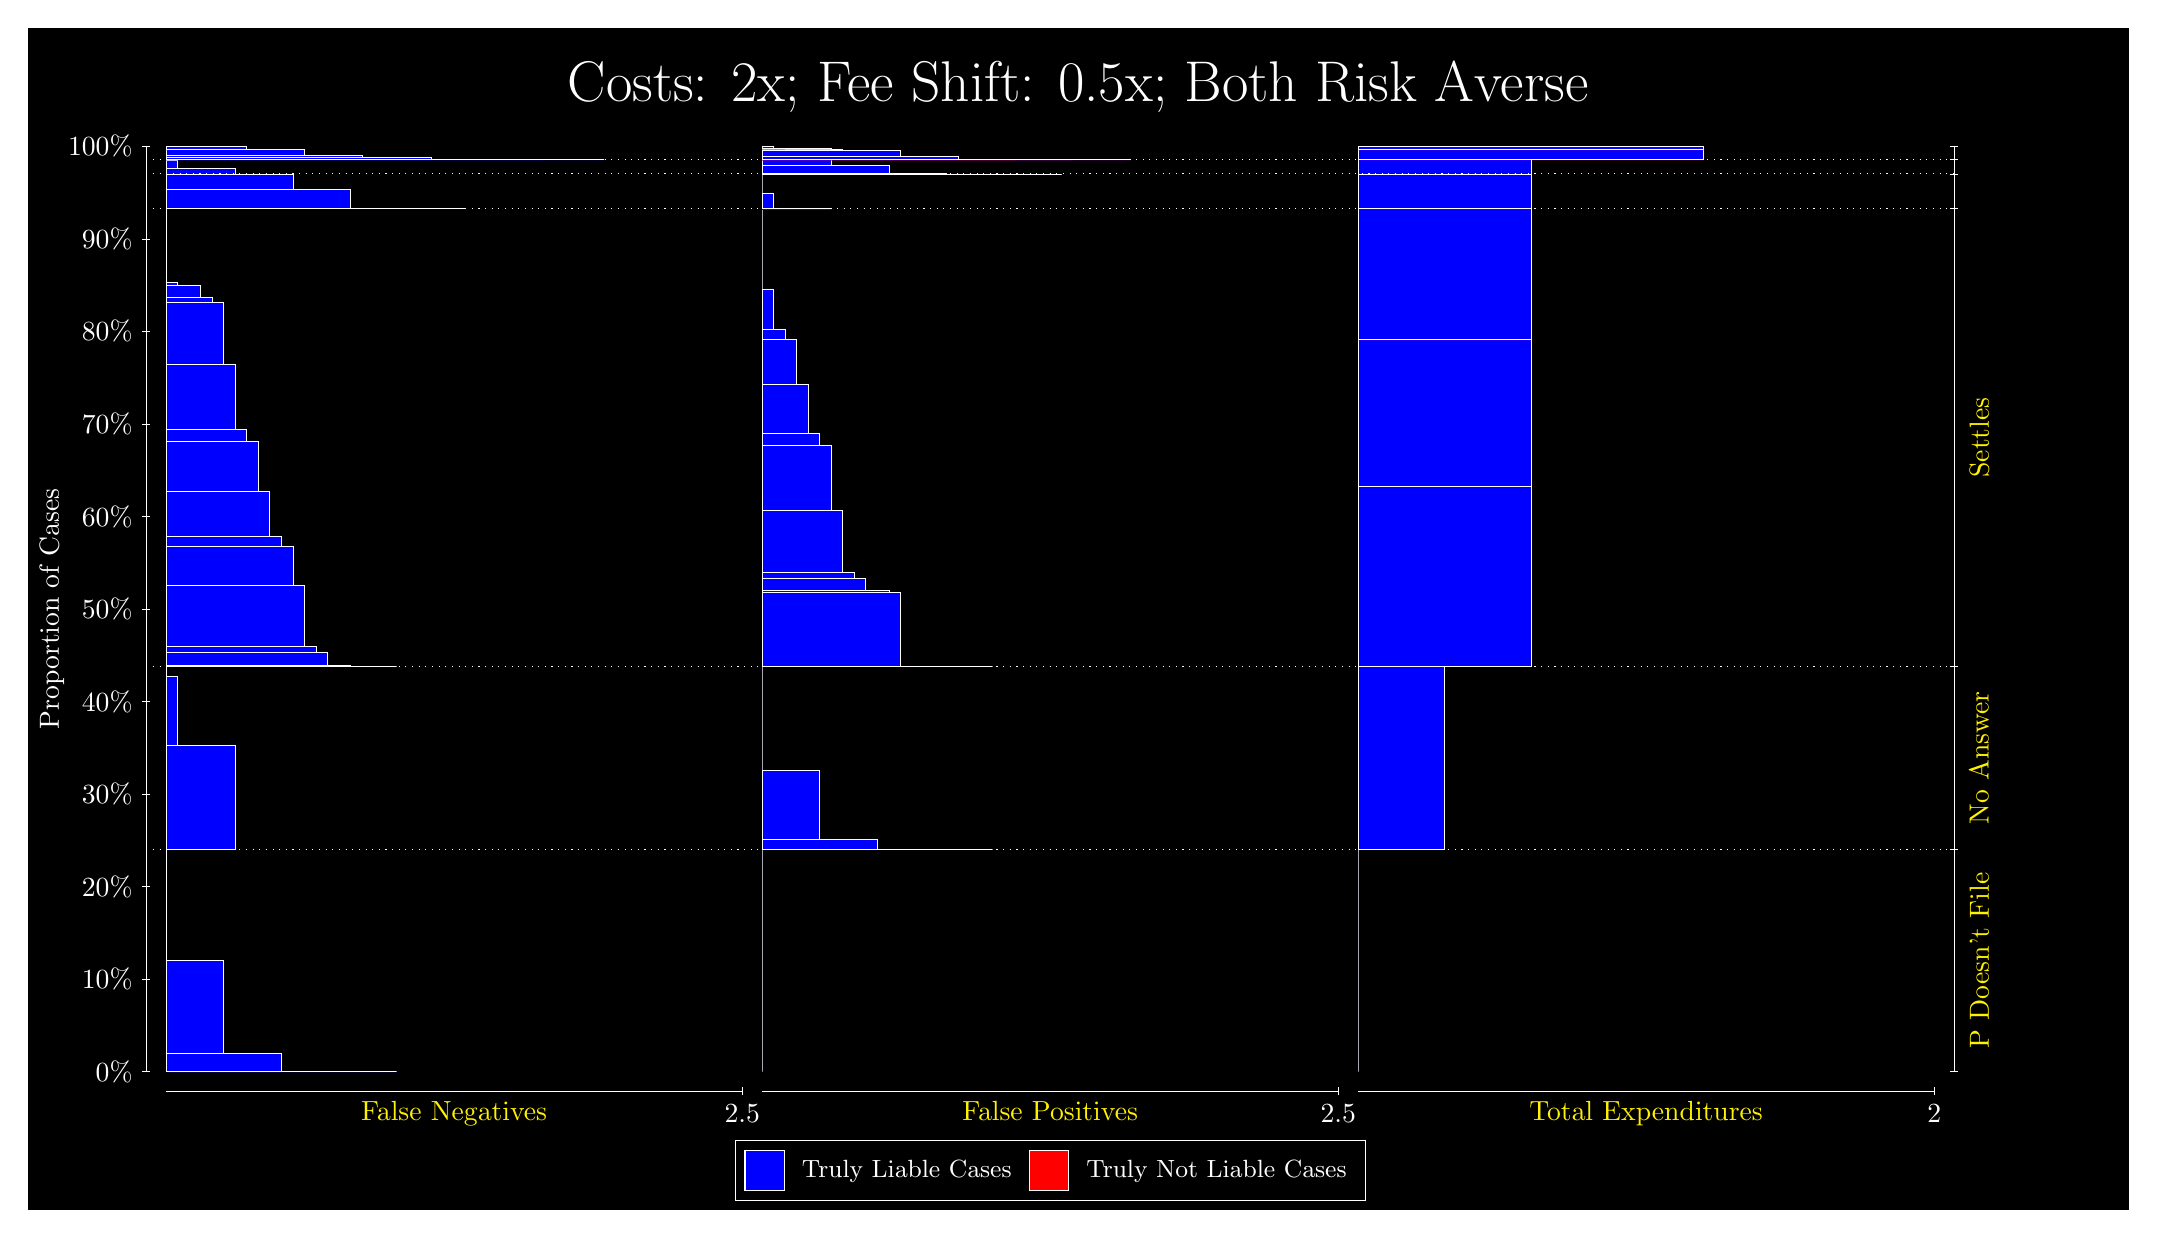
\begin{tikzpicture}
\draw[fill=black] (0,0) rectangle (26.667,15);
\draw[text=white] (0,13.5) rectangle (26.667,15) node[midway] {\huge Costs: 2x; Fee Shift: 0.5x; Both Risk Averse};
\draw[white, very thin] (1.5,1.75) -- (1.5,13.5);
\node[rotate=90, text=white, anchor=center] at (0.3, 7.625) {Proportion of Cases};
\draw[white, very thin] (1.45,1.75) -- (1.55,1.75);
\node[text=white, anchor=east] at (1.45, 1.75) {0\%};
\draw[white, very thin] (1.45,2.925) -- (1.55,2.925);
\node[text=white, anchor=east] at (1.45, 2.925) {10\%};
\draw[white, very thin] (1.45,4.1) -- (1.55,4.1);
\node[text=white, anchor=east] at (1.45, 4.1) {20\%};
\draw[white, very thin] (1.45,5.275) -- (1.55,5.275);
\node[text=white, anchor=east] at (1.45, 5.275) {30\%};
\draw[white, very thin] (1.45,6.45) -- (1.55,6.45);
\node[text=white, anchor=east] at (1.45, 6.45) {40\%};
\draw[white, very thin] (1.45,7.625) -- (1.55,7.625);
\node[text=white, anchor=east] at (1.45, 7.625) {50\%};
\draw[white, very thin] (1.45,8.8) -- (1.55,8.8);
\node[text=white, anchor=east] at (1.45, 8.8) {60\%};
\draw[white, very thin] (1.45,9.975) -- (1.55,9.975);
\node[text=white, anchor=east] at (1.45, 9.975) {70\%};
\draw[white, very thin] (1.45,11.15) -- (1.55,11.15);
\node[text=white, anchor=east] at (1.45, 11.15) {80\%};
\draw[white, very thin] (1.45,12.325) -- (1.55,12.325);
\node[text=white, anchor=east] at (1.45, 12.325) {90\%};
\draw[white, very thin] (1.45,13.5) -- (1.55,13.5);
\node[text=white, anchor=east] at (1.45, 13.5) {100\%};

\draw[white, very thin] (24.457,1.75) -- (24.457,13.5);
\draw[white, very thin] (24.407,1.75) -- (24.507,1.75);
\node[anchor=west] at (24.407, 1.75) {};
\draw[white, very thin] (24.407,4.5712) -- (24.507,4.5712);
\node[anchor=west] at (24.407, 4.5712) {};
\draw[white, very thin] (24.407,6.895) -- (24.507,6.895);
\node[anchor=west] at (24.407, 6.895) {};
\draw[white, very thin] (24.407,12.708) -- (24.507,12.708);
\node[anchor=west] at (24.407, 12.708) {};
\draw[white, very thin] (24.407,13.15) -- (24.507,13.15);
\node[anchor=west] at (24.407, 13.15) {};
\draw[white, very thin] (24.407,13.332) -- (24.507,13.332);
\node[anchor=west] at (24.407, 13.332) {};
\draw[white, very thin] (24.407,13.5) -- (24.507,13.5);
\node[anchor=west] at (24.407, 13.5) {};

\draw[white, very thin, fill=blue] (1.75,1.75) rectangle (4.6775,1.75);
\draw[white, very thin, fill=blue] (1.75,1.75) rectangle (3.9457,1.7522);
\draw[white, very thin, fill=blue] (1.75,1.7522) rectangle (3.2138,1.9772);
\draw[white, very thin, fill=blue] (1.75,1.9772) rectangle (2.4819,3.1635);
\draw[white, very thin, fill=red] (1.75,3.1635) rectangle (1.75,3.1635);
\draw[white, very thin, fill=blue] (1.75,3.1635) rectangle (1.75,4.5712);
\draw[white, very thin, fill=blue] (1.75,4.5712) rectangle (2.6283,5.8936);
\draw[white, very thin, fill=blue] (1.75,5.8936) rectangle (1.8964,6.7666);
\draw[white, very thin, fill=red] (1.75,6.7666) rectangle (1.75,6.7666);
\draw[white, very thin, fill=blue] (1.75,6.7666) rectangle (1.75,6.895);
\draw[white, very thin, fill=blue] (1.75,6.895) rectangle (4.6775,6.895);
\draw[white, very thin, fill=blue] (1.75,6.895) rectangle (4.3848,6.8952);
\draw[white, very thin, fill=blue] (1.75,6.8952) rectangle (4.092,6.9107);
\draw[white, very thin, fill=blue] (1.75,6.9107) rectangle (3.9457,6.9111);
\draw[white, very thin, fill=blue] (1.75,6.9111) rectangle (3.7993,7.0778);
\draw[white, very thin, fill=blue] (1.75,7.0778) rectangle (3.6529,7.1524);
\draw[white, very thin, fill=blue] (1.75,7.1524) rectangle (3.5065,7.9234);
\draw[white, very thin, fill=blue] (1.75,7.9234) rectangle (3.3602,8.4214);
\draw[white, very thin, fill=blue] (1.75,8.4214) rectangle (3.2138,8.5523);
\draw[white, very thin, fill=blue] (1.75,8.5523) rectangle (3.0674,9.1224);
\draw[white, very thin, fill=blue] (1.75,9.1224) rectangle (2.921,9.7513);
\draw[white, very thin, fill=blue] (1.75,9.7513) rectangle (2.7746,9.9053);
\draw[white, very thin, fill=blue] (1.75,9.9053) rectangle (2.6283,10.726);
\draw[white, very thin, fill=blue] (1.75,10.726) rectangle (2.4819,11.517);
\draw[white, very thin, fill=blue] (1.75,11.517) rectangle (2.3355,11.587);
\draw[white, very thin, fill=blue] (1.75,11.587) rectangle (2.1891,11.737);
\draw[white, very thin, fill=blue] (1.75,11.737) rectangle (2.0428,11.739);
\draw[white, very thin, fill=blue] (1.75,11.739) rectangle (1.8964,11.768);
\draw[white, very thin, fill=red] (1.75,11.768) rectangle (1.75,11.768);
\draw[white, very thin, fill=blue] (1.75,11.768) rectangle (1.75,12.708);
\draw[white, very thin, fill=blue] (1.75,12.708) rectangle (5.5558,12.708);
\draw[white, very thin, fill=blue] (1.75,12.708) rectangle (4.8239,12.713);
\draw[white, very thin, fill=blue] (1.75,12.713) rectangle (4.092,12.957);
\draw[white, very thin, fill=blue] (1.75,12.957) rectangle (3.3602,13.148);
\draw[white, very thin, fill=blue] (1.75,13.148) rectangle (2.6283,13.15);
\draw[white, very thin, fill=red] (1.75,13.15) rectangle (1.75,13.15);
\draw[white, very thin, fill=blue] (1.75,13.15) rectangle (2.6283,13.222);
\draw[white, very thin, fill=blue] (1.75,13.222) rectangle (1.8964,13.325);
\draw[white, very thin, fill=red] (1.75,13.325) rectangle (1.75,13.325);
\draw[white, very thin, fill=blue] (1.75,13.325) rectangle (1.75,13.332);
\draw[white, very thin, fill=blue] (1.75,13.332) rectangle (7.3123,13.332);
\draw[white, very thin, fill=blue] (1.75,13.332) rectangle (6.5805,13.332);
\draw[white, very thin, fill=blue] (1.75,13.332) rectangle (5.8486,13.336);
\draw[white, very thin, fill=blue] (1.75,13.336) rectangle (5.7022,13.336);
\draw[white, very thin, fill=blue] (1.75,13.336) rectangle (5.1167,13.36);
\draw[white, very thin, fill=blue] (1.75,13.36) rectangle (4.9703,13.36);
\draw[white, very thin, fill=blue] (1.75,13.36) rectangle (4.3848,13.366);
\draw[white, very thin, fill=blue] (1.75,13.366) rectangle (4.2384,13.381);
\draw[white, very thin, fill=blue] (1.75,13.381) rectangle (3.6529,13.381);
\draw[white, very thin, fill=blue] (1.75,13.381) rectangle (3.5065,13.459);
\draw[white, very thin, fill=blue] (1.75,13.459) rectangle (2.921,13.459);
\draw[white, very thin, fill=blue] (1.75,13.459) rectangle (2.7746,13.498);
\draw[white, very thin, fill=blue] (1.75,13.498) rectangle (2.0428,13.5);
\draw[white, very thin, fill=red] (1.75,13.5) rectangle (1.75,13.5);
\draw[white, very thin, fill=blue] (1.75,13.5) rectangle (1.75,13.5);
\draw[white, very thin, fill=red] (9.3189,1.75) rectangle (9.3189,1.75);
\draw[white, very thin, fill=blue] (9.3189,1.75) rectangle (9.3189,4.5712);
\draw[white, very thin, fill=red] (9.3189,4.5712) rectangle (12.246,4.5712);
\draw[white, very thin, fill=blue] (9.3189,4.5712) rectangle (12.246,4.5712);
\draw[white, very thin, fill=blue] (9.3189,4.5712) rectangle (11.515,4.5714);
\draw[white, very thin, fill=blue] (9.3189,4.5714) rectangle (10.783,4.6997);
\draw[white, very thin, fill=blue] (9.3189,4.6997) rectangle (10.051,5.5727);
\draw[white, very thin, fill=blue] (9.3189,5.5727) rectangle (9.3189,6.895);
\draw[white, very thin, fill=red] (9.3189,6.895) rectangle (12.246,6.895);
\draw[white, very thin, fill=blue] (9.3189,6.895) rectangle (12.246,6.895);
\draw[white, very thin, fill=red] (9.3189,6.895) rectangle (11.954,6.895);
\draw[white, very thin, fill=blue] (9.3189,6.895) rectangle (11.954,6.895);
\draw[white, very thin, fill=red] (9.3189,6.895) rectangle (11.661,6.895);
\draw[white, very thin, fill=blue] (9.3189,6.895) rectangle (11.661,6.895);
\draw[white, very thin, fill=blue] (9.3189,6.895) rectangle (11.515,6.895);
\draw[white, very thin, fill=red] (9.3189,6.895) rectangle (11.368,6.895);
\draw[white, very thin, fill=blue] (9.3189,6.895) rectangle (11.368,6.8965);
\draw[white, very thin, fill=blue] (9.3189,6.8965) rectangle (11.222,6.8966);
\draw[white, very thin, fill=red] (9.3189,6.8966) rectangle (11.075,6.8966);
\draw[white, very thin, fill=blue] (9.3189,6.8966) rectangle (11.075,7.8351);
\draw[white, very thin, fill=blue] (9.3189,7.8351) rectangle (10.929,7.8645);
\draw[white, very thin, fill=blue] (9.3189,7.8645) rectangle (10.783,7.866);
\draw[white, very thin, fill=blue] (9.3189,7.866) rectangle (10.636,8.016);
\draw[white, very thin, fill=blue] (9.3189,8.016) rectangle (10.49,8.0864);
\draw[white, very thin, fill=blue] (9.3189,8.0864) rectangle (10.344,8.8768);
\draw[white, very thin, fill=blue] (9.3189,8.8768) rectangle (10.197,9.6978);
\draw[white, very thin, fill=blue] (9.3189,9.6978) rectangle (10.051,9.8518);
\draw[white, very thin, fill=blue] (9.3189,9.8518) rectangle (9.9044,10.481);
\draw[white, very thin, fill=blue] (9.3189,10.481) rectangle (9.758,11.051);
\draw[white, very thin, fill=blue] (9.3189,11.051) rectangle (9.6116,11.182);
\draw[white, very thin, fill=blue] (9.3189,11.182) rectangle (9.4652,11.68);
\draw[white, very thin, fill=blue] (9.3189,11.68) rectangle (9.3189,12.708);
\draw[white, very thin, fill=red] (9.3189,12.708) rectangle (10.197,12.708);
\draw[white, very thin, fill=blue] (9.3189,12.708) rectangle (10.197,12.71);
\draw[white, very thin, fill=blue] (9.3189,12.71) rectangle (9.4652,12.901);
\draw[white, very thin, fill=blue] (9.3189,12.901) rectangle (9.3189,13.15);
\draw[white, very thin, fill=red] (9.3189,13.15) rectangle (13.125,13.15);
\draw[white, very thin, fill=blue] (9.3189,13.15) rectangle (13.125,13.15);
\draw[white, very thin, fill=blue] (9.3189,13.15) rectangle (12.393,13.15);
\draw[white, very thin, fill=blue] (9.3189,13.15) rectangle (11.661,13.158);
\draw[white, very thin, fill=blue] (9.3189,13.158) rectangle (10.929,13.26);
\draw[white, very thin, fill=blue] (9.3189,13.26) rectangle (10.197,13.332);
\draw[white, very thin, fill=red] (9.3189,13.332) rectangle (14.003,13.332);
\draw[white, very thin, fill=blue] (9.3189,13.332) rectangle (14.003,13.332);
\draw[white, very thin, fill=red] (9.3189,13.332) rectangle (13.271,13.332);
\draw[white, very thin, fill=blue] (9.3189,13.332) rectangle (13.271,13.332);
\draw[white, very thin, fill=red] (9.3189,13.332) rectangle (12.539,13.332);
\draw[white, very thin, fill=blue] (9.3189,13.332) rectangle (12.539,13.335);
\draw[white, very thin, fill=blue] (9.3189,13.335) rectangle (11.807,13.373);
\draw[white, very thin, fill=red] (9.3189,13.373) rectangle (11.807,13.373);
\draw[white, very thin, fill=blue] (9.3189,13.373) rectangle (11.807,13.373);
\draw[white, very thin, fill=red] (9.3189,13.373) rectangle (11.661,13.373);
\draw[white, very thin, fill=blue] (9.3189,13.373) rectangle (11.661,13.373);
\draw[white, very thin, fill=blue] (9.3189,13.373) rectangle (11.075,13.45);
\draw[white, very thin, fill=blue] (9.3189,13.45) rectangle (11.075,13.451);
\draw[white, very thin, fill=red] (9.3189,13.451) rectangle (10.929,13.451);
\draw[white, very thin, fill=blue] (9.3189,13.451) rectangle (10.929,13.451);
\draw[white, very thin, fill=blue] (9.3189,13.451) rectangle (10.344,13.459);
\draw[white, very thin, fill=blue] (9.3189,13.459) rectangle (10.344,13.466);
\draw[white, very thin, fill=blue] (9.3189,13.466) rectangle (10.197,13.472);
\draw[white, very thin, fill=red] (9.3189,13.472) rectangle (10.197,13.472);
\draw[white, very thin, fill=blue] (9.3189,13.472) rectangle (10.197,13.472);
\draw[white, very thin, fill=blue] (9.3189,13.472) rectangle (9.6116,13.472);
\draw[white, very thin, fill=blue] (9.3189,13.472) rectangle (9.6116,13.472);
\draw[white, very thin, fill=blue] (9.3189,13.472) rectangle (9.4652,13.496);
\draw[white, very thin, fill=blue] (9.3189,13.496) rectangle (9.4652,13.496);
\draw[white, very thin, fill=blue] (9.3189,13.496) rectangle (9.3189,13.5);
\draw[white, very thin, fill=red] (16.888,1.75) rectangle (16.888,1.75);
\draw[white, very thin, fill=blue] (16.888,1.75) rectangle (16.888,4.5712);
\draw[white, very thin, fill=red] (16.888,4.5712) rectangle (17.986,4.5712);
\draw[white, very thin, fill=blue] (16.888,4.5712) rectangle (17.986,6.895);
\draw[white, very thin, fill=red] (16.888,6.895) rectangle (19.083,6.895);
\draw[white, very thin, fill=blue] (16.888,6.895) rectangle (19.083,9.1853);
\draw[white, very thin, fill=red] (16.888,9.1853) rectangle (19.083,9.1853);
\draw[white, very thin, fill=blue] (16.888,9.1853) rectangle (19.083,11.046);
\draw[white, very thin, fill=red] (16.888,11.046) rectangle (19.083,11.046);
\draw[white, very thin, fill=blue] (16.888,11.046) rectangle (19.083,12.708);
\draw[white, very thin, fill=red] (16.888,12.708) rectangle (19.083,12.708);
\draw[white, very thin, fill=blue] (16.888,12.708) rectangle (19.083,13.15);
\draw[white, very thin, fill=red] (16.888,13.15) rectangle (19.083,13.15);
\draw[white, very thin, fill=blue] (16.888,13.15) rectangle (19.083,13.332);
\draw[white, very thin, fill=red] (16.888,13.332) rectangle (21.279,13.332);
\draw[white, very thin, fill=blue] (16.888,13.332) rectangle (21.279,13.458);
\draw[white, very thin, fill=red] (16.888,13.458) rectangle (21.279,13.458);
\draw[white, very thin, fill=blue] (16.888,13.458) rectangle (21.279,13.5);
\draw[white, dotted] (1.5,4.5712) -- (24.457,4.5712);
\draw[white, dotted] (1.5,6.895) -- (24.457,6.895);
\draw[white, dotted] (1.5,12.708) -- (24.457,12.708);
\draw[white, dotted] (1.5,13.15) -- (24.457,13.15);
\draw[white, dotted] (1.5,13.332) -- (24.457,13.332);
\draw[white, very thin] (1.75,1.5) -- (9.0689,1.5);
\node[text=yellow, anchor=north] at (5.4094, 1.5) {False Negatives};
\draw[white, very thin] (9.0689,1.45) -- (9.0689,1.55);
\node[text=white, anchor=north] at (9.0689, 1.45) {2.5};

\draw[white, very thin] (9.3189,1.5) -- (16.638,1.5);
\node[text=yellow, anchor=north] at (12.978, 1.5) {False Positives};
\draw[white, very thin] (16.638,1.45) -- (16.638,1.55);
\node[text=white, anchor=north] at (16.638, 1.45) {2.5};

\draw[white, very thin] (16.888,1.5) -- (24.207,1.5);
\node[text=yellow, anchor=north] at (20.547, 1.5) {Total Expenditures};
\draw[white, very thin] (24.207,1.45) -- (24.207,1.55);
\node[text=white, anchor=north] at (24.207, 1.45) {2};

\node[text=yellow, centered, rotate=90] at (24.777, 3.1606) {P Doesn't File};
\node[text=yellow, centered, rotate=90] at (24.777, 5.7331) {No Answer};
\node[text=yellow, centered, rotate=90] at (24.777, 9.8016) {Settles};




\draw (12.978300999999998,1.5) node[draw=none] (baseCoordinate) {};
\begin{scope}[align=center]
        \matrix[scale=0.5, draw=white, below=0.5cm of baseCoordinate, nodes={draw}, column sep=0.1cm]{
            \node[rectangle, draw, minimum width=0.5cm, minimum height=0.5cm, fill=blue] {}; &
            \node[draw=none, font=\small, text=white] (B) {Truly Liable Cases}; &
            \node[rectangle, draw, minimum width=0.5cm, minimum height=0.5cm, fill=red] {}; &
            \node[draw=none, font=\small, text=white] (B) {Truly Not Liable Cases}; \\
            };
\end{scope}

\end{tikzpicture}
\end{document}